%-------------------------------------------------------------------------------
% File:		    Proposal.tex
% Author:	    Igor Janjic, Danny Duangphachanh, Daniel Friedman
% Description:	[ECE 4564] Network Applications Design
%		        Project proposal report.
%%------------------------------------------------------------------------------ 

%-------------------------------------------------------------------------------
% File:		Preamble.tex
% Author:	Igor Janjic
% Description:	Defines which packages to use.
%%------------------------------------------------------------------------------

\documentclass[11pt]{article}

% Encodes font as T1.
\usepackage[T1]{fontenc}

% Pretty much all of the ams maths packages.
\usepackage{amsmath,amsthm,amssymb,amsfonts}

% Allows you to manipulate the page a bit.
\usepackage[margin=0.75in]{geometry}

% Removes paragraph indentation.
\usepackage{parskip}

% Allows inclusion of graphics easily.
\usepackage{graphicx}

% Provides ways to make nice looking tables.
\usepackage{booktabs}

% Allows rotation of tables and figures.
\usepackage{rotating}

% Allows color.
\usepackage{color}

% Allows shading of table cells.
\usepackage{colortbl}

% Allows hyphenatable letterspacing, underlining, and highlighting.
\usepackage{soul}

% Allows extra text symbols.
\usepackage{textcomp}

% Allows manipulation of floats.
\usepackage{float}

% Provides commands to make subfigures.
\usepackage{subfigure}

% Typesets URLs sensibly with tt font, clickability in PDFs, and not breaking across lines.
\usepackage{url}

% Makes references hyperlinks in PDF output.
\usepackage{hyperref}

% Provides good access to colors.
\usepackage{color}

% Provides good access to colors.
\usepackage{xcolor}

% Provides for programming code to be inserted into the document.
\usepackage{listings}

% Provides support for table coloring.
\usepackage{xcolor}

% Provides vector graphics functionality.
\usepackage{tikz}
\usetikzlibrary{shapes.geometric, arrows, positioning}

% Provides circuit vector graphics functionality.
\usepackage{circuitikz}

% Provides caption manipulation.
\usepackage{caption}

% Makes sure tables don't float about if they have the designation [H].
\restylefloat{table}

% Defines the color gray.
\definecolor{gray}{rgb}{0.5, 0.5, 0.5}


%-------------------------------------------------------------------------------
% File:		Definitions.tex
% Author:	Igor Janjic
% Description:	Contains various commands.
%%------------------------------------------------------------------------------

%-------------------------------------------------------------------------------
% General Definitions

% Defines a command for skipping a line.
\def\wl{\par\vspace{\baselineskip}}

% Defines a command for hiding text.
\newcommand{\hide}[1]{}

% Defines a command for a shortened commonly used phrases.
\newcommand{\ie}{\text{i.e.}}
\newcommand{\eg}{\text{e.g.}}
\newcommand{\ex}{\text{e.x.}}
\newcommand{\ans}{\textbf{Answer: }}
\newcommand{\pro}{\textbf{Proof: }}

% Defines a command to mark to-do items in red.
\newcommand{\todo}[1] {\textbf{\textcolor{red}{#1}}}

% Defines commands for calligraphic font.
\newcommand{\calA}{\mathcal{A}}
\newcommand{\calB}{\mathcal{B}}
\newcommand{\calC}{\mathcal{C}}
\newcommand{\calD}{\mathcal{D}}
\newcommand{\calE}{\mathcal{E}}
\newcommand{\calF}{\mathcal{F}}
\newcommand{\calG}{\mathcal{G}}
\newcommand{\calH}{\mathcal{H}}
\newcommand{\calI}{\mathcal{I}}
\newcommand{\calJ}{\mathcal{J}}
\newcommand{\calK}{\mathcal{K}}
\newcommand{\calL}{\mathcal{L}}
\newcommand{\calM}{\mathcal{M}}
\newcommand{\calN}{\mathcal{N}}
\newcommand{\calO}{\mathcal{O}}
\newcommand{\calP}{\mathcal{P}}
\newcommand{\calQ}{\mathcal{Q}}
\newcommand{\calR}{\mathcal{R}}
\newcommand{\calS}{\mathcal{S}}
\newcommand{\calT}{\mathcal{T}}
\newcommand{\calU}{\mathcal{U}}
\newcommand{\calV}{\mathcal{V}}
\newcommand{\calW}{\mathcal{W}}
\newcommand{\calX}{\mathcal{X}}
\newcommand{\calY}{\mathcal{Y}}
\newcommand{\calZ}{\mathcal{Z}}

% Defines commands for bold font.
\newcommand{\bbA}{\mathbb{A}}
\newcommand{\bbB}{\mathbb{B}}
\newcommand{\bbC}{\mathbb{C}}
\newcommand{\bbD}{\mathbb{D}}
\newcommand{\bbE}{\mathbb{E}}
\newcommand{\bbF}{\mathbb{F}}
\newcommand{\bbG}{\mathbb{G}}
\newcommand{\bbH}{\mathbb{H}}
\newcommand{\bbI}{\mathbb{I}}
\newcommand{\bbJ}{\mathbb{J}}
\newcommand{\bbK}{\mathbb{K}}
\newcommand{\bbL}{\mathbb{L}}
\newcommand{\bbM}{\mathbb{M}}
\newcommand{\bbN}{\mathbb{N}}
\newcommand{\bbO}{\mathbb{O}}
\newcommand{\bbP}{\mathbb{P}}
\newcommand{\bbQ}{\mathbb{Q}}
\newcommand{\bbR}{\mathbb{R}}
\newcommand{\bbS}{\mathbb{S}}
\newcommand{\bbT}{\mathbb{T}}
\newcommand{\bbU}{\mathbb{U}}
\newcommand{\bbV}{\mathbb{V}}
\newcommand{\bbW}{\mathbb{W}}
\newcommand{\bbX}{\mathbb{X}}
\newcommand{\bbY}{\mathbb{Y}}
\newcommand{\bbZ}{\mathbb{Z}}

% Defines commands for bold face font.
\newcommand{\bfA}{\mathbf{A}}
\newcommand{\bfB}{\mathbf{B}}
\newcommand{\bfC}{\mathbf{C}}
\newcommand{\bfD}{\mathbf{D}}
\newcommand{\bfE}{\mathbf{E}}
\newcommand{\bfF}{\mathbf{F}}
\newcommand{\bfG}{\mathbf{G}}
\newcommand{\bfH}{\mathbf{H}}
\newcommand{\bfI}{\mathbf{I}}
\newcommand{\bfJ}{\mathbf{J}}
\newcommand{\bfK}{\mathbf{K}}
\newcommand{\bfL}{\mathbf{L}}
\newcommand{\bfM}{\mathbf{M}}
\newcommand{\bfN}{\mathbf{N}}
\newcommand{\bfO}{\mathbf{O}}
\newcommand{\bfP}{\mathbf{P}}
\newcommand{\bfQ}{\mathbf{Q}}
\newcommand{\bfR}{\mathbf{R}}
\newcommand{\bfS}{\mathbf{S}}
\newcommand{\bfT}{\mathbf{T}}
\newcommand{\bfU}{\mathbf{U}}
\newcommand{\bfV}{\mathbf{V}}
\newcommand{\bfW}{\mathbf{W}}
\newcommand{\bfX}{\mathbf{X}}
\newcommand{\bfY}{\mathbf{Y}}
\newcommand{\bfZ}{\mathbf{Z}}

% Defines commands for lists.
\newcommand{\be}{\begin{enumerate}}
\newcommand{\ee}{\end{enumerate}}
\newcommand{\ba}{\begin{align}}
\newcommand{\ea}{\end{align}}
\newcommand{\bas}{\begin{align*}}
\newcommand{\eassss}{\end{align*}}

%-------------------------------------------------------------------------------
% Math Definitions

% Defines a command for a function.
\newcommand{\func}[2]{#1 \left( #2 \right)}

% Defines a command for an integral.
\newcommand{\dint}[4]{\int_{#1}^{#2}#3\;d#4}

% Defines commands for objects.
\newcommand{\csum}[2]{\sum_{#1}^{#2}}
\newcommand{\cint}[2]{\int_{#1}{#2}}
\newcommand{\cprod}[2]{\prod_{#1}^{#2}}

% Defines commands for various parentheses.
\newcommand{\paren}[1]{\left( #1 \right)}
\newcommand{\sqprn}[1]{\left[ #1 \right]}
\newcommand{\tlprn}[1]{\left\{ #1 \right\}}

% Defines a command for the absolute value of an expression.
\newcommand{\abs}[1]{\left| #1 \right|}

% Defines commands for various angled expressions.
\newcommand{\tr}[2]{\left<\left< #1 , #2 \right>\right>}
\newcommand{\trs}[2]{\left< #1 , #2 \right>}
\newcommand{\iprod}[2]{\left\langle #1 , #2 \right\rangle}

% Defines commands for various deltas.
\newcommand{\del}{\partial}
\newcommand{\dd}[2]{\frac{d#1}{d#2}}
\newcommand{\ddel}[2]{\frac{\del#1}{\del#2}}
\newcommand{\ddell}[2]{\frac{\del^2#1}{{\del#2}^2}}
\newcommand{\ddelll}[3]{\frac{\del^2#1}{{\del#2}{\del#3}}}

% Defines a command for evaluating an expression at a particular value.
\newcommand{\eval}[3]{\left.#1\right|_{#2}^{#3}}

% Defines commands for flooring and ceiling.
\newcommand{\ceil}[1]{\ensuremath{\left\lceil#1\right\rceil}}
\newcommand{\floor}[1]{\ensuremath{\left\lfloor#1\right\rfloor}}

% Defines commands for argmin and argmax.
\newcommand{\argmin}{\mathop{\mathrm{argmin}}}
\newcommand{\argmax}{\mathop{\mathrm{argmax}}}

% Defines a command for mapping.
\newcommand{\map}{\mathop{\mathrm{map}}}

% Defines a command for an inverse.
\newcommand{\inv}{^{-1}}

% Defines a command for the partial derivative operator.
\newcommand{\pd}[2]{\frac{\partial #1}{\partial #2}}

% Defines commands for function names.
\newcommand{\zeros}{\mathrm{zeros}}
\newcommand{\rank}{\mathrm{rank}}
\newcommand{\TR}{\mathrm{tr}}
\newcommand{\vol}{\mathrm{vol}}
\newcommand{\sgn}{\mathrm{sgn}}
\newcommand{\acos}{\mathrm{acos}}
\newcommand{\intr}{\mathrm{int}\,}
\newcommand{\extr}{\mathrm{ext}\,}
\newcommand{\dom}{\mathrm{dom}\,}
\newcommand{\conv}{\mathrm{conv}\hspace{1pt}}
\newcommand{\cone}{\mathrm{cone}\hspace{1pt}}

% Defines commands for symbols in probability and statistics.
\newcommand{\convd}{\overset{{\scriptsize d}}{\to}}
\newcommand{\convp}{\overset{{\scriptsize p}}{\to}}
\newcommand{\unif}{\mathrm{Uniform}}
\newcommand{\bern}{\mathrm{Bernoulli}}
\newcommand{\negbin}{\mathrm{NegBinom}}
\newcommand{\Binom}{\mathrm{Bin}}
\newcommand{\pois}{\mathrm{Poisson}}
\newcommand{\ndistr}{\mathrm{n}}
\newcommand{\Bdistr}{\mathrm{Beta}}
\newcommand{\Gdistr}{\mathrm{Gamma}}
\newcommand{\iGdistr}{\mathrm{InvGamma}}
\newcommand{\MSE}{\mathrm{MSE}}
\newcommand{\MAE}{\mathrm{MAE}}
\newcommand{\ARE}{\mathrm{ARE}}
\newcommand{\se}{\mathrm{se}}
\newcommand{\mexp}{\text{{\bf E}}}
\newcommand{\var}{\mathrm{Var}}
\newcommand{\cov}{\mathrm{Cov}}
\newcommand{\corr}{\mathrm{Cor}}
\newcommand{\bW}{\bs{W}}
\newcommand{\bw}{\bs{w}}
\newcommand{\bX}{\bs{X}}
\newcommand{\bx}{\bs{x}}
\newcommand{\bY}{\bs{Y}}
\newcommand{\by}{\bs{y}}
\newcommand{\bZ}{\bs{Z}}
\newcommand{\bz}{\bs{z}}
\newcommand{\Xbar}{\overline{X}}
\newcommand{\ev}{\mathrm{Ev}}
\newcommand{\pr}{\boldsymbol{\mathrm{P}}}


%-------------------------------------------------------------------------------
% File:		Programming.tex
% Author:	Igor Janjic
% Description:	Defines programming environments.
%%------------------------------------------------------------------------------

\lstnewenvironment{matlab}{
\lstset{
    	language = matlab,	
	basicstyle = \footnotesize\ttfamily,
	numbers = left,
	numberstyle = \tiny\color{gray},
	stepnumber = 1,
	numbersep = 5pt,
 	backgroundcolor = \color{white},
 	showspaces = false,
  	showstringspaces = false,
  	showtabs = false,
  	frame = single,
  	rulecolor = \color{black},
  	tabsize = 4,
  	breaklines = true,
  	breakatwhitespace = false,
  	title = \lstname,
    	upquote = true,
    	aboveskip = {1.5\baselineskip},
    	columns=fixed,
   	extendedchars = true,
   	prebreak = \raisebox{0ex}[0ex][0ex]{\ensuremath{\hookleftarrow}},
    	identifierstyle=\ttfamily,
    	keywordstyle=\color[rgb]{0,0,1},
    	commentstyle=\color[rgb]{0.133,0.545,0.133},
    	stringstyle=\color[rgb]{0.627,0.126,0.941}
}}{}

\lstnewenvironment{tex}{
\lstset{
    	language = TeX,	
	basicstyle = \footnotesize\ttfamily,
	numbers = left,
	numberstyle = \tiny\color{gray},
	stepnumber = 1,
	numbersep = 5pt,
 	backgroundcolor = \color{white},
 	showspaces = false,
  	showstringspaces = false,
  	showtabs = false,
  	frame = shadowbox,
  	rulecolor = \color{black},
  	tabsize = 4,
  	breaklines = true,
  	breakatwhitespace = false,
  	title = \lstname,
    	upquote = true,
    	aboveskip = {1.5\baselineskip},
    	columns=fixed,
   	extendedchars = true,
    	identifierstyle=\ttfamily,
	xleftmargin=0.5cm,
	xrightmargin=0.5cm,
    	keywordstyle=\color[rgb]{0,0,1},
    	commentstyle=\color[rgb]{0.133,0.545,0.133},
    	stringstyle=\color[rgb]{0.627,0.126,0.941}
}}{}

\lstnewenvironment{pseudo}{
\lstset{
	basicstyle = \footnotesize,
	numbers = left,
	numberstyle = \tiny\color{gray},
	stepnumber = 1,
	numbersep = 5pt,
 	backgroundcolor = \color{white},
 	showspaces = false,
  	showstringspaces = false,
  	showtabs = false,
  	frame = single,
  	rulecolor = \color{black},
  	tabsize = 4,
  	captionpos = b,
  	breaklines = true,
  	breakatwhitespace = false,
  	title = \lstname,
    	upquote = true,
    	aboveskip = {1.5\baselineskip},
    	columns=fixed,
   	extendedchars = true,
   	prebreak = \raisebox{0ex}[0ex][0ex]{\ensuremath{\hookleftarrow}},
}}{}



% Make compact sections.
\usepackage[compact]{titlesec}

\begin{document}

%-------------------------------------------------------------------------------
% File:		    Title.tex
% Author:	    Igor Janjic
% Description:	[ECE 4564] Network Applications Design
%		        Project proposal.
%%------------------------------------------------------------------------------

\begin{titlepage}

\centering
\vspace*{\baselineskip}

\rule{\textwidth}{1.6pt}\vspace*{-\baselineskip}\vspace*{2pt}
\rule{\textwidth}{0.4pt}\\[\baselineskip]

{\LARGE PROJECT PROPOSAL\\[0.3\baselineskip]
PiFeed -- Feed Your Pets with a Raspberry Pi\\[0.2\baselineskip]
 }

\rule{\textwidth}{0.4pt}\vspace*{-\baselineskip}\vspace{3.2pt}
\rule{\textwidth}{1.6pt}\\[\baselineskip]

\wl

\scshape Due November 9, 2014 at 11:55 PM.
{\small 
\\[\baselineskip]\par}

\vfill

Created by:\\[0.2\baselineskip]
{Danny Duangphachanh: \texttt{ijanjic@vt.edu}}\\[0.2\baselineskip]
{Daniel Friedman:     \texttt{ijanjic@vt.edu}}\\[0.2\baselineskip]
{Igor Janjic:         \texttt{ijanjic@vt.edu}}\\[0.4\baselineskip]
{\small \today}\\[0.8\baselineskip]
{\small [ECE 4564] Network Applications Design}\\[0.2\baselineskip]
{\small\itshape Virginia Polytechnic Institute and\\ State University}\\[0.2\baselineskip]

\begin{center}
	
\includegraphics[scale=0.35]{images/Logo}
\end{center}

\end{titlepage}


\section{Concept of Operations}
The purpose of PiFeed is to be able to remotely monitor and control a fish tank
and cat feeder from the internet. The system will be composed of two
Raspberry Pi's and one computer. Rasp1 will collect information about the fish
tank and control the fish feeder. Rasp2 will collect information about the cat
and control the cat feeder. A user will interface with the two Raspberry Pi's
with a client application and be able to monitor both the aquarium and the cat
feeder using Pi cameras. Additionally the client application will allow the user
to customize the feeders and control them manually. We will consider the system
successful if our pets can be fed remotely. The ability to maintain a healthy
eating schedule for pets is a concern for members of our group, as well as many
others who travel or are away from home for an extended amount of time. By
euccessfully implementing a pet feeding and monitoring system using Raspberry
Pis, the stresses of animal care while away will be a thing of the past! A
high level overview of Rasp1 is described in Figure~\ref{fig:highFish} and of
Rasp2 in Figure~\ref{fig:highCat}.

\begin{figure}[H]
    \centering
    \begin{minipage}[b]{0.45\linewidth}
        \centering
        \captionsetup{justification=centering, margin = 0.5cm}
        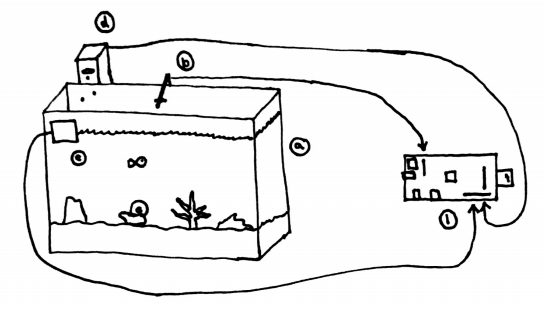
\includegraphics[scale=0.3]{images/FishTank} 
        \caption{Diagram of Rasp1. (a) Aquarium. (b) Pi camera used for
        monitoring fish. (c) Sensors used for monitoring aquarium environment.
        (d) Automatic fish food feeder.}
        \label{fig:highFish}
    \end{minipage}
    \quad
    \begin{minipage}[b]{0.45\linewidth}
        \centering
        \captionsetup{justification=centering, margin = 0.5cm}
        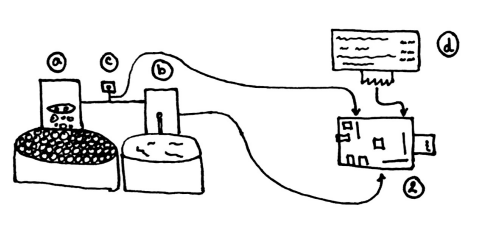
\includegraphics[scale=0.4]{images/Cat} 
        \caption{Diagram of Rasp2. (a) Automatic cat food feeder and sensors.
        (b) Automatic cat water feeder (c) Pi camera used for monitoring cat.
        (d) LCD display.}
        \label{fig:highCat}
    \end{minipage}
\end{figure}

\section{System Overview}
PiFeed is separated into the following modules: PiFeedControl, PiFeedFish, and
PiFeedCat. The programming language that will be used is Python. Rabbitmq will
be used for publishing the sensor information and images from both the fish tank
and cat bowls to a message broker that the PiFeedControl client application can
subscribe to. The Rabbitmq server will be located on a machine on the same
network that Rasp1 and Rasp2 are connected on. Python sockets will be used for
controlling the feeders remotely and the LCD connected to Rasp2.

\subsection{PiFeedControl}
The purpose of this module is to be able to allow a user to remotely access and
control the feeders as well as write messages to the LCD display connected to
Rasp2. The module is a python client application and can be run using either the
local network or the internet. It will talk to PiFeedCat and PiFeedFish by
subscribing to a message broker that routes the messages from the two modules.
It will use sockets to manually start the feeders and configure the feeders for
automatic feeding as well as for writing to the LCD display connected to Rasp2.

\subsection{PiFeedCat}
The purpose of this module is to publish messages to a message broker containing
information generated by the sensors on the cat bowls as well as images from the
Pi camera mounted on the bowls. It also controls the hardware for the automatic
cat feeder and the LCD.

\subsection{PiFeedFish}
The purpose of this module is to publish messages to a message broker containing
information generated by the sensors on the fish tank as well as images from the
Pi camera mounted on the tank. It also controls the hardware for the automatic
fish tank feeder.

\subsection{Testable Requirements}
A completely successful project should demonstrate that the following requirements
are satisfied.
\begin{enumerate}
    \item PiFeedControl is able to remotely feed the fish both manually and at
          specific times of the day.
    \item PiFeedControl is able to remotely feed the cat both manually and at
          specific times of the day.
    \item PiFeedControl is able to remotely monitor the fish using the Pi camera.
    \item PiFeedControl is able to remotely monitor the cat using the Pi camera.
    \item PiFeedControl is able to remotely view the fish tank sensors.
    \item PiFeedControl is able to remotely view the cat sensors.
    \item PiFeedFish is able to feed the fish.
    \item PiFeedFish is able to interface with the sensors on the fish tank and
          get correct readings.
    \item PiFeedCat is able to feed the cat.
    \item PiFeedCat is able to interface with the sensors on the cat bowls and
          get correct readings.
\end{enumerate}

\subsection{Use Case Diagram}

\begin{figure}[H]
    \centering
    \captionsetup{justification=centering, margin = 0.5cm}
    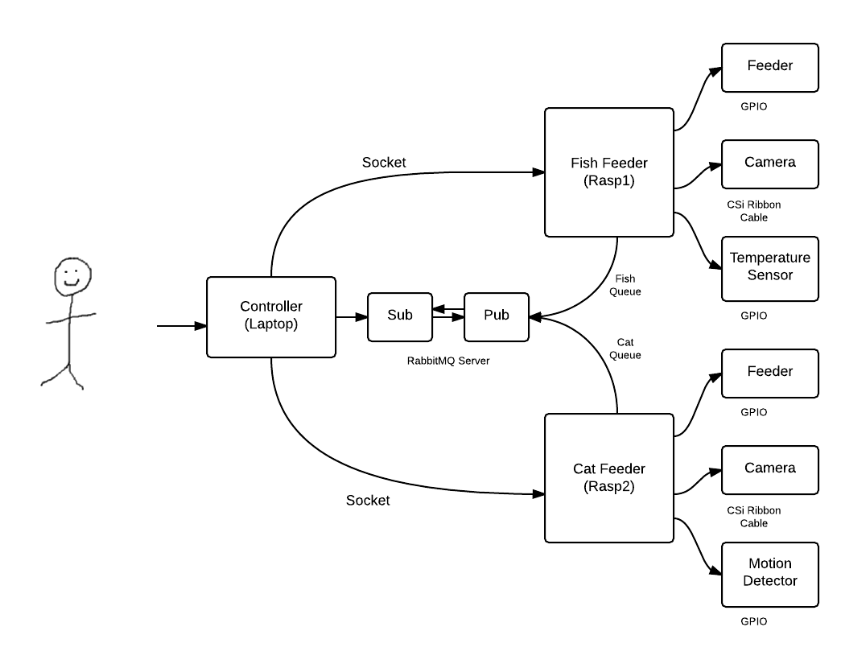
\includegraphics[scale=0.4]{images/UseCase} 
    \caption{Use case diagram for the entire system. A user interfaces with a
    client program on a laptop that connects to a RabbitMQ message broker to
    remotely monitor the fish tank and cat. Sockets allow the controller to
    configure feeders and manually control them as well as to write messages to
    the LCD connected.}
    \label{fig:UseCase}
\end{figure}

Figure~\ref{fig:UseCase} shows the different users that will be interacting with
the system. A user interfaces withe the whole system using a command line
application called PiFeedControl. This application subscribes to an exchange on
a RabbitMQ server containing two different message queues, one for each feeder.
PiFeedControl will then be able to receive messages from the pi's containing both
the readings of the sensors and images from the cameras on the Pi's. PiFeedControl
will also be able to configure the feeders and manually control them using a
custom socket protocol.

\section{Hardware List}
\begin{enumerate}
    \item 2 Raspberry Pi boards (borrowing already)
    \item 2 SD cards (16GB) (borrowing already)
    \item 2 WiFi + Bluetooth 3.0 USB adaptors (borrowing already)
    \item 2 MicroUSB cables (borrowing already)
    \item 2 USB chargers (borrowing already)
    \item 2 5MP camera board modules (owned)
    \item Cheap Pi LCD display (need to borrow)
    \item Servos (owned)
    \item Jumper wires (need to borrow)
    \item DS18B20 waterproof temperature sensor (need to borrow)
    \item Adafruit PIR Motion Sensor (need to borrow)

\end{enumerate}

\section{GitHub Details}
\begin{tabular}{ l c l c l}
    \textbf{Team Member} & :: & \textbf{PID} & :: & \textbf{GitHub} \\
    Daniel Friedman      & :: & adfriedm     & :: & adfriedm        \\
    Danny Duangphachanh  & :: & bboydd       & :: & daduang         \\
    Igor Janjic          & :: & ijanjic      & :: & zergler
\end{tabular}

\section{Project Schedule}

\subsection{Development Tasks}
\begin{enumerate}
    \item Get hardware components (Everyone)
    \item Set up fish tank and get a cat food and water bowl (Igor)
    \item Design fish tank automated feeder (Everyone)
    \item Design cat automated feeder (Everyone)
    \item Build fish tank automated feeder design (Everyone)
    \item Build cat automated feeder (Everyone)
    \item Connect hardware components (Danny)
    \item Write PiFeedControl python module (Igor)
    \item Write PiFeedCat python module (Danny)
    \item Write PiFeedFish python module (Daniel)
    \item Test all hardware component interfaces (Everyone)
    \item Test PiFeedControl python module interface (Everyone)
    \item Test PiFeedFish (Everyone)
    \item Test PiFeedCat (Everyone)
    \item Test communication between PiFeedCat and PiFeedFish with
          PiFeedControler (Everyone)
    \item Beta build demonstration (Everyone)
    \item Final demonstration (Everyone)

\end{enumerate}

\subsection{Milestones}
\begin{enumerate}
    \item Beta build demonstration (12-01-14): For the beta build demonstration,
    we will demonstrate that the raspberry pi can collect images from both
    raspberry pi's and send them to the controller client program using
    RabbitMQ.
    \item Final demonstration (12-16-14): For the final demonstration, we will
    show that we have satisfied all of our requirements.
\end{enumerate}

\begin{figure}{H}
    \centering
    \captionsetup{justification=centering, margin = 0.5cm}
    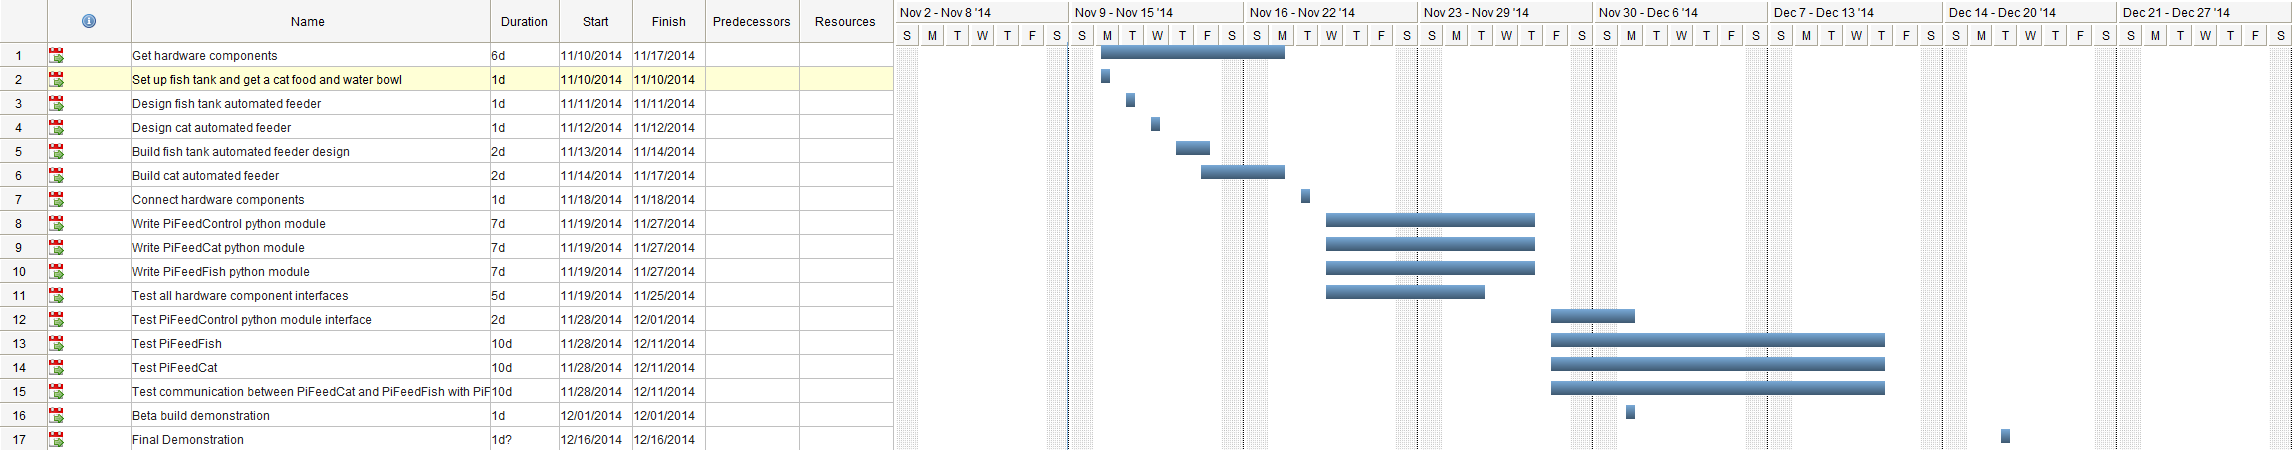
\includegraphics[scale=0.3]{images/Gant} 
    \caption{Gant chart of the proposed schedule.}
    \label{fig:gant}
\end{figure}


\end{document}
